\documentclass[12pt]{article}
\usepackage[left=1cm, right=1cm, top=2cm,bottom=1.5cm]{geometry} 

\usepackage[parfill]{parskip}
\usepackage[utf8]{inputenc}
\usepackage[T2A]{fontenc}
\usepackage[russian]{babel}
\usepackage{enumitem}
\usepackage[normalem]{ulem}
\usepackage{amsfonts, amsmath, amsthm, amssymb, mathtools,xcolor,accents}
\usepackage{blkarray}

\usepackage{tabularx}
\usepackage{hhline}

\usepackage{accents}
\usepackage{fancyhdr}
\pagestyle{fancy}
\renewcommand{\headrulewidth}{1.5pt}
\renewcommand{\footrulewidth}{1pt}

\usepackage{graphicx}
\usepackage[figurename=Рис.]{caption}
\usepackage{subcaption}
\usepackage{float}

%%Наименование папки откуда забирать изображения
\graphicspath{ {./images/} }

%%Изменение формата для ввода доказательства
\renewcommand{\proofname}{$\square$  \nopunct}
\renewcommand\qedsymbol{$\blacksquare$}

%%Изменение отступа на таблицах
\addto\captionsrussian{%
	\renewcommand{\proofname}{$\square$ \nopunct}%
}
%% Римские цифры
\newcommand{\RN}[1]{%
	\textup{\uppercase\expandafter{\romannumeral#1}}%
}

%% Для удобства записи
\newcommand{\MR}{\mathbb{R}}
\newcommand{\MC}{\mathbb{C}}
\newcommand{\MQ}{\mathbb{Q}}
\newcommand{\MN}{\mathbb{N}}
\newcommand{\MZ}{\mathbb{Z}}
\newcommand{\MTB}{\mathbb{T}}
\newcommand{\MTI}{\mathbb{I}}
\newcommand{\MI}{\mathrm{I}}
\newcommand{\MCI}{\mathcal{I}}
\newcommand{\MJ}{\mathrm{J}}
\newcommand{\MH}{\mathrm{H}}
\newcommand{\MT}{\mathrm{T}}
\newcommand{\MU}{\mathcal{U}}
\newcommand{\MV}{\mathcal{V}}
\newcommand{\MB}{\mathcal{B}}
\newcommand{\MF}{\mathcal{F}}
\newcommand{\MW}{\mathcal{W}}
\newcommand{\ML}{\mathcal{L}}
\newcommand{\MP}{\mathcal{P}}
\newcommand{\VN}{\varnothing}
\newcommand{\VE}{\varepsilon}
\newcommand{\dx}{\, dx}
\newcommand{\dy}{\, dy}
\newcommand{\dz}{\, dz}
\newcommand{\dd}{\, d}


\theoremstyle{definition}
\newtheorem{defn}{Опр:}
\newtheorem{rem}{Rm:}
\newtheorem{prop}{Утв.}
\newtheorem{exrc}{Упр.}
\newtheorem{problem}{Задача}
\newtheorem{lemma}{Лемма}
\newtheorem{theorem}{Теорема}
\newtheorem{corollary}{Следствие}

\newenvironment{cusdefn}[1]
{\renewcommand\thedefn{#1}\defn}
{\enddefn}

\DeclareRobustCommand{\divby}{%
	\mathrel{\text{\vbox{\baselineskip.65ex\lineskiplimit0pt\hbox{.}\hbox{.}\hbox{.}}}}%
}
\DeclareRobustCommand{\ndivby}{\mkern-1mu\not\mathrel{\mkern4.5mu\divby}\mkern1mu}


%Короткий минус
\DeclareMathSymbol{\SMN}{\mathbin}{AMSa}{"39}
%Длинная шапка
\newcommand{\overbar}[1]{\mkern 1.5mu\overline{\mkern-1.5mu#1\mkern-1.5mu}\mkern 1.5mu}
%Функция знака
\DeclareMathOperator{\sgn}{sgn}

%Функция ранга
\DeclareMathOperator{\rk}{\text{rk}}
\DeclareMathOperator{\diam}{\text{diam}}


%Обозначение константы
\DeclareMathOperator{\const}{\text{const}}

\DeclareMathOperator{\codim}{\text{codim}}

\DeclareMathOperator*{\dsum}{\displaystyle\sum}
\newcommand{\ddsum}[2]{\displaystyle\sum\limits_{#1}^{#2}}
\newcommand{\ddssum}[2]{\displaystyle\smashoperator{\sum\limits_{#1}^{#2}}}
\newcommand{\ddlsum}[2]{\displaystyle\smashoperator[l]{\sum\limits_{#1}^{#2}}}
\newcommand{\ddrsum}[2]{\displaystyle\smashoperator[r]{\sum\limits_{#1}^{#2}}}

%Интеграл в большом формате
\DeclareMathOperator{\dint}{\displaystyle\int}
\newcommand{\ddint}[2]{\displaystyle\int\limits_{#1}^{#2}}
\newcommand{\ssum}[1]{\displaystyle \sum\limits_{n=1}^{\infty}{#1}_n}

\newcommand{\smallerrel}[1]{\mathrel{\mathpalette\smallerrelaux{#1}}}
\newcommand{\smallerrelaux}[2]{\raisebox{.1ex}{\scalebox{.75}{$#1#2$}}}

\newcommand{\smallin}{\smallerrel{\in}}
\newcommand{\smallnotin}{\smallerrel{\notin}}

\newcommand*{\medcap}{\mathbin{\scalebox{1.25}{\ensuremath{\cap}}}}%
\newcommand*{\medcup}{\mathbin{\scalebox{1.25}{\ensuremath{\cup}}}}%

\makeatletter
\newcommand{\vast}{\bBigg@{3.5}}
\newcommand{\Vast}{\bBigg@{5}}
\makeatother

%Промежуточное значение для sup\inf, поскольку они имеют разную высоту
\newcommand{\newsup}{\mathop{\smash{\mathrm{sup}}}}
\newcommand{\newinf}{\mathop{\mathrm{inf}\vphantom{\mathrm{sup}}}}

%Скалярное произведение
\newcommand{\inner}[2]{\left\langle #1, #2 \right\rangle }
\newcommand{\linsp}[1]{\left\langle #1 \right\rangle }
\newcommand{\linmer}[2]{\left\langle #1 \vert #2\right\rangle }

%Подпись символов снизу
\newcommand{\ubar}[1]{\underaccent{\bar}{#1}}

%%Шапка для букв сверху
\newcommand{\wte}[1]{\widetilde{#1}}
\newcommand{\wht}[1]{\widehat{#1}}
\newcommand{\ovl}[1]{\overline{#1}}


%%Трансформация Фурье
\newcommand{\fourt}[1]{\mathcal{F}\left(#1\right)}
\newcommand{\ifourt}[1]{\mathcal{F}^{-1}\left(#1\right)}

%%Символ вектора
\newcommand{\vecm}[1]{\overrightarrow{#1\,}}

%%Пространстов матриц
\newcommand{\matsq}[1]{\operatorname{Mat}_{#1}}
\newcommand{\mat}[2]{\operatorname{Mat}_{#1, #2}}

%Оператор для действ и мнимых чисел
\DeclareMathOperator{\IM}{\operatorname{Im}}
\DeclareMathOperator{\RE}{\operatorname{Re}}
\DeclareMathOperator{\li}{\operatorname{li}}
\DeclareMathOperator{\GL}{\operatorname{GL}}
\DeclareMathOperator{\SL}{\operatorname{SL}}
\DeclareMathOperator{\Char}{\operatorname{char}}
\DeclareMathOperator\Arg{Arg}
\DeclareMathOperator\ord{ord}

%Оператор для образа
\DeclareMathOperator{\Ima}{Im}

%Делимость чисел
\newcommand{\modn}[3]{#1 \equiv #2 \; (\bmod \; #3)}
\newcommand{\nmodn}[3]{#1 \not\equiv #2 \; (\bmod \; #3)}

%%Взятие в скобки, модули и норму
\newcommand{\parfit}[1]{\left( #1 \right)}
\newcommand{\modfit}[1]{\left| #1 \right|}
\newcommand{\sqparfit}[1]{\left\{ #1 \right\}}
\newcommand{\normfit}[1]{\left\| #1 \right\|}

%%Функция для обозначения равномерной сходимости по множеству
\newcommand{\uconv}[1]{\overset{#1}{\rightrightarrows}}
\newcommand{\uconvm}[2]{\overset{#1}{\underset{#2}{\rightrightarrows}}}

%% Функция для добавления круга сверху множества
\newcommand{\Circ}[1]{\accentset{\circ}{#1}}

%%Функция для обозначения нижнего и верхнего интегралов
\def\upint{\mathchoice%
	{\mkern13mu\overline{\vphantom{\intop}\mkern7mu}\mkern-20mu}%
	{\mkern7mu\overline{\vphantom{\intop}\mkern7mu}\mkern-14mu}%
	{\mkern7mu\overline{\vphantom{\intop}\mkern7mu}\mkern-14mu}%
	{\mkern7mu\overline{\vphantom{\intop}\mkern7mu}\mkern-14mu}%
	\int}
\def\lowint{\mkern3mu\underline{\vphantom{\intop}\mkern7mu}\mkern-10mu\int}

%%След матрицы
\DeclareMathOperator*{\tr}{tr}

\makeatletter
\renewcommand*\env@matrix[1][*\c@MaxMatrixCols c]{%
	\hskip -\arraycolsep
	\let\@ifnextchar\new@ifnextchar
	\array{#1}}
\makeatother


%% Переопределение функции хи, чтобы выглядела более приятно
\makeatletter
\@ifdefinable\@latex@chi{\let\@latex@chi\chi}
\renewcommand*\chi{{\@latex@chi\smash[t]{\mathstrut}}} % want only bottom half of \mathstrut
\makeatletter

\setcounter{MaxMatrixCols}{20}

\begin{document}
\lhead{Математический анализ - \RN{4}}
\chead{Шапошников С.В.}
\rhead{Лекция - 7}
\section*{Формула замены переменных}
\begin{theorem}(\textbf{Формула замены переменных})
	Пусть $\Omega_x, \Omega_y \subset \MR^n$ - открытые и ограниченные множества. $\varphi \colon \Omega_x \to \Omega_y$ - диффеоморфизм, $\ovl{E}\subset \Omega_x$ и $E$ - допустимое множество. Пусть $f \colon \varphi(E) \to \MR$, тогда функция $f$ интегрируема по Риману на $\varphi(E) \Leftrightarrow f(\varphi(x)){\cdot}|\det{\MJ_\varphi(x)}|$ интегрируема на $E$ и в случае интегрируемости верно равенство:
	$$
		\ddint{\varphi(E)}{}f(y)dy = \ddint{E}{}f(\varphi(x)){\cdot}|\det{\MJ_\varphi(x)}|dx
	$$
\end{theorem}
\begin{rem}
	Не обязательно, чтобы $\Omega_x, \Omega_y \subset \MR^n$ были ограниченными, поскольку сама теорема будет верна для допустимых множеств.
\end{rem}
\begin{proof}\hfill\\	
	\uline{Проверка формулы в частном случае $2)$}:	
	$$
		\varphi \colon \Omega_x = \MR^n \to \Omega_y =\MR^n, \, \varphi(x) = Ax + b, \, \det(A) \neq 0
	$$ 
	Множество $E$ это брус или образ бруса при невырожденном аффинном преобразовании (как $\varphi$). Пусть $f$ будет непрерывна на $\MR^n$. Проверим равенство:
	$$
		\ddint{\varphi(E)}{}f(y)dy = \ddint{E}{}f(\varphi(x)){\cdot}|\det{(A)}|dx
	$$
	
	\begin{lemma}
		Всякое отображение: $\varphi(x) = Ax + b$ является композицией конечного набора отображений следующего вида:\hfill
		\begin{enumerate}[label=(\arabic*)]
			\item Переставление координат (смотри случай $1)$);
			\item $y_1 = x_1, \dotsc , y_{n-1} = x_{n-1}, y_n = x_n + c$, где $c$ - какое-то число;
			\item $y_1 = x_1, \dotsc , y_{n-1} = x_{n-1}, y_n = c{\cdot}x_n$, где $c$ - какое-то число;
			\item $y_1 = x_1, \dotsc , y_{n-1} = x_{n-1}, y_n = x_n + x_{n-1}$;
		\end{enumerate}
		То есть $\varphi = \varphi_1 \circ \varphi_2 \circ \dotsc \circ \varphi_m$, где каждое отображение является одного из этих видов.
	\end{lemma}
	\begin{proof}
		$(1)$ и $(2) \Rightarrow$ далее считаем $b = 0 \Rightarrow \varphi(x) = Ax$. Вспомним, что $E_{ij}$ - матрица, где на $(i,j)$-м месте стоит $1$ и $0$ на всех остальных, то есть матричная единица. Тогда:
		$$
			(I + E_{ij})A = A + A_{ij}, \, i \neq j
		$$
		где $A_{ij}$ это матрица состоящая из $j$-ой строки матрицы $A$ на $i$-ом месте $\Rightarrow$ мы получили прибавление к $i$-ой строке $j$-ой строки. Рассмотрим матрицу $E_i^c$ - матрица полученная из единичной, домножением на $c$ единицы на $(i,i)$-м месте. Тогда $E_i^c{\cdot}A$ - домножение $i$-ой строчки на $c$. Следовательно, мы умеем складывать строки и умножать на числа $\Rightarrow$ мы умеем переставлять строчки местами:
		$$
			\begin{pmatrix}
				i\\
				j
			\end{pmatrix} \xrightarrow[ i + j]{}
			\begin{pmatrix}
				i \\
				i + j
			\end{pmatrix} \xrightarrow[ j - (i + j)]{}
			\begin{pmatrix}
				-j\\
				i + j
			\end{pmatrix} \xrightarrow[ i+ j + (-j)]{}
			\begin{pmatrix}
				-j\\
				i
			\end{pmatrix} \xrightarrow[ \cdot (-1)]{}
			\begin{pmatrix}
				j\\
				i
			\end{pmatrix}
		$$
		Умножая матрицу $A$ на матрицы $E_1, \dotsc, E_m$ мы можем привести её к единичной матрице:
		$$
			E_m{\cdot}E_{m-1}{\cdot}\dotsc{\cdot}E_2{\cdot}E_1{\cdot}A = I
		$$
		Также заметим, что обратные преобразования - это преобразования такого же вида, тогда:
		$$
			A = E^{-1}_1{\cdot}\dotsc{\cdot}E^{-1}_m = \wte{E}_1{\cdot}\dotsc{\cdot}\wte{E}_m
		$$
		Аналогично, при умножении таких матриц на вектора: $E_{ij}{\cdot}x \Rightarrow x_i \to x_i + x_j$ и $E_i^c{\cdot}x \Rightarrow x_i \to c{\cdot}x_i$. Таким образом, мы представили: $\varphi(x) = A{\cdot}x$ в виде композиций отображений вида: $x_i{\cdot}c$ или $x_i + x_j$, где остальные координаты остаются на местах. С учетом возможности перестановки координат, лемма доказана.
	\end{proof}
	Применим теорему Фубини и проверим, что для каждого из преобразований $(2), (3), (4)$ верна ФЗП:
	$$
		\varphi = \varphi_1 \circ \varphi_2 \circ \dotsc \circ \varphi_m, \, \ddint{\varphi(E)}{}f(y)dy = \ddint{\varphi_2{\circ}\dotsc{\circ}\varphi_m(E)}{}f(\varphi_1(z)){\cdot}|\varphi'_1(z)|dz =  \dotsc = 
	$$
	$$
		= \ddint{E}{}f(\varphi_1{\circ}\varphi_2{\circ}\dotsc{\circ}\varphi_m(x)){\cdot}|\varphi'_1|{\cdot}|\varphi'_2|{\cdot}\dotsc{\cdot}|\varphi'_m|dx = \ddint{E}{}f(\varphi(x)){\cdot}|\varphi'|dx
	$$
	Таким образом, достаточно проверить для каждого из простых преобразований верность формулы выше. Проверим для $(4)$ (аналогично для $(2)$ и $(3)$):
	$$
		\varphi \colon y_1 = x_1, \dotsc, y_{n-1} = x_{n-1}, y_n = x_n + x_{n-1}
	$$
	Мы знаем, что $E$ это заведомо допустимое множество: брус или его образ аффинного преобразования, в частности это выпуклое множество, его одномерные сечения это промежутки, а поскольку $E$ - ограничено, то это ограниченные промежутки (либо интервал, либо полуинтервал, либо отрезок). Если $f$ всюду непрерывна, то всё можно интегрировать по этим сечениям. Пусть верно:
	$$
		E \subset \MI_{n-1}\times [a_n,b_n], \, \ovl{E} \subset \Circ{\MI}_{n-1} \times (a_n,b_n) \Rightarrow
	$$
	$$
		\Rightarrow \varphi(E) \subset \{(y_1,\dotsc, y_n) \mid (y_1, \dotsc, y_{n-1}) \in \MI_{n-1}, \, a_n + y_{n-1} \leq y_n \leq b_n + y_{n-1}  \}
	$$
	Поскольку $y_1, \dotsc, y_{n-1}$ бегают по бруску, то: 
	$$
		\exists \, A,B \colon E,\, \varphi(E) \subset \Circ{\MI}_{n-1} \times (A,B) \Rightarrow \ddint{\varphi(E)}{}f(y_1,\dotsc, y_n)dy_1{\cdot}\dotsc{\cdot}dy_n = \ddint{\MI_{n-1} \times [A,B]}{}f(y)\chi_{\varphi(E)}(y)dy 
	$$
	Применяем теорему Фубини и мы получим:
	$$
		\ddint{\MI_{n-1} \times [A,B]}{}f(y)\chi_{\varphi(E)}(y)dy  = \ddint{\MI_{n-1}}{}dy_1{\cdot}\dotsc{\cdot}dy_{n-1} \ddint{A}{B}f(y_1,\dotsc, y_{n-1}, y_n){\cdot}\chi_{\varphi(E)}(y_1,\dotsc, y_{n-1},y_n)dy_n = 
	$$
	$$
		= \ddint{\MI_{n-1}}{}dx_1{\cdot}\dotsc{\cdot}dx_{n-1}\ddint{A}{B}f(x_1,\dotsc,x_{n-1},y_n){\cdot}\chi_{\varphi(E)}(x_1,\dotsc, x_{n-1},y_n)dy_n 
	$$
	Далее, мы делаем замену $y_n = x_n + x_{n-1}$ в одномерном интеграле, которую мы умеем делать из второго семестра:
	$$
		\ddint{A}{B}f(x_1,\dotsc,x_{n-1},y_n){\cdot}\chi_{\varphi(E)}(x_1,\dotsc, x_{n-1},y_n)dy_n  =
	$$
	$$	
		= \ddint{A - x_{n-1}}{B - x_{n-1}}f(x_1,\dotsc,x_{n-1},x_n + x_{n-1}){\cdot}\chi_{\varphi(E)}(x_1,\dotsc, x_{n-1},x_n + x_{n-1})dx_n = (*)
	$$
	где $\chi_{\varphi(E)}(x_1,\dotsc, x_{n-1},x_n + x_{n-1} = \chi_{\varphi(E)}(\varphi(x)) = \chi_E(x)$, поскольку $\varphi$ - диффеоморфизм. Далее, поскольку мы выбрали $A$ и $B$ столь большими, что: $E \subset \MI_{n-1}\times [A - x_{n-1},B - x_{n-1}]$, тогда:
	$$
		[A - x_{n-1},B - x_{n-1}] \subset [A,B] \Rightarrow (*) = \ddint{A}{B}f(x_1,\dotsc,x_{n-1},x_n + x_{n-1})\chi_{E}(x_1,\dotsc,x_n)dx_n \Rightarrow  
	$$
	$$
		\Rightarrow \ddint{\varphi(E)}{}f(y)dy =  \ddint{\MI_{n-1}}{}dx_1{\cdot}\dotsc{\cdot}dx_{n-1}\ddint{A}{B}f(x_1,\dotsc,x_{n-1}, x_{n} + x_{n-1})\chi_E(x)dx_n = 
	$$
	$$
		= \ddint{\MI_{n-1}}{}dx_1{\cdot}\dotsc{\cdot}dx_{n-1}\ddint{A}{B}f(\varphi(x))\chi_E(x)dx_n = \ddint{E}{}f(\varphi(x))dx
	$$
	где в последнем равенстве мы опять воспользовались теоремой Фубини. Это является правильной формулой замены переменной, поскольку для такого преобразования: $|\varphi'| = 1$.
\end{proof}
\begin{rem}
	Как доказывается вся ФЗП с помощью такого же приема - смотри Зорич, второй том.
\end{rem}
\begin{rem}
	Общий случай будет разобран позднее и сразу для интеграла Лебега, но из того, что мы доказали уже следует полезное равенство: $E$ это брус, $\varphi(x) = Ax + b, \, \det{(A)} \neq 0$, то тогда:
	$$
		|\varphi(E)| = |\det{(A)}|{\cdot}|E|
	$$
	Чтобы получить это равенство, надо в доказанном взять $f = 1$. Смысл этой формулы: объем параллелепипеда равен определителю матрицы, задающей вектора параллелепипеда, умноженному на объем бруса из которого этот параллелепипед получается.
\end{rem}
\begin{corollary}
	Значение интеграла Римана не зависит от выбора декартовой системы координат.
\end{corollary}
\begin{proof}
	Пусть изначально были координаты в $\MR^n$ - $x$, которые мы ортогональным преобразованием заменили на $y$. Поскольку преобразование ортогональное, то определитель $\varphi$ равен единице и верно равенство:
	$$
		\ddint{E_x}{}f(x)dx = \ddint{E_y}{}f(y)dy
	$$
\end{proof}
\begin{rem}
	Заметим, что если начнутся какие-либо растяжения, менять объемы, то значения интеграла также будут меняться. Поэтому речь идет только об ортонормированных системах координат.
\end{rem}
\newpage
\section*{Применение формулы замены переменной}
\subsection*{Теорема Брауэра}
\begin{theorem}(\textbf{Брауэра})
	Если $f$ - непрерывное отображение замкнутого шара: $\ovl{\MB} \to \ovl{\MB}$, то:
	$$
		\exists \, x \in \ovl{\MB} \colon f(x) = x
	$$
\end{theorem}
\begin{rem}
	Доказательство предложил Милнер. Следствие теоремы Брауэра - теорема Шаудера.
\end{rem}
\begin{proof}
	Начнём со случая, когда $f \colon \MR^n \to \MR^n$ - гладкое отображение. Для определенности возьмем единичный шар: $\MB = \MB(0,1)$, $f\colon \ovl{\MB} \to \ovl{\MB}$. Обычно первая часть доказательства всегда сводится к лемме о барабане: нельзя стянуть полотно барабана не разорвав на границе. Предположим, что $f(x) \neq x$ на $\ovl{\MB}$, тогда проведём луч через $f(x)$ и $x$ до пересечения с границей:
	$$
		F(x) = x + \lambda(x){\cdot}(x - f(x)), \quad \lambda(x) \colon \|F(x)\| = 1
	$$
	\begin{figure}[H]
		\centering
		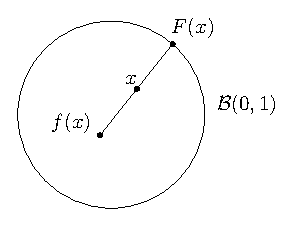
\includegraphics[width=0.25\textwidth]{MA4L7_1.eps}
		\caption{Построение $F(x)$.}
		\label{7_1}
	\end{figure}
	Мы ожидаем от него следующее:
	\begin{enumerate}[label=(\arabic*)]
		\item $F(x)$ - гладкая в $\MB(0,1 + \delta), \, \delta > 0$;
		\item $\|F(x)\| = 1$, то есть: $F \colon \ovl{\MB}(0,1) \to \partial \MB(0,1)$;
		\item (\uline{Ретракция}): $\forall x \in \partial \MB(0,1), \, F(x) = x$;
	\end{enumerate}
	\textbf{\uline{Идея}}: Из того, что $f(x) \neq x$, мы построим такое отображение $F(x)$, а затем с помощью ФЗП поймем, что такого отображения не существует и придём к противоречию. То, что такого отображения не существует и называется леммой о барабане/леммой об отсутствии ретракции шара на свою границу.
	$$
		1 = \|F(x)\|^2 = \|x + \lambda{\cdot}(x - f(x))\|^2 = \|x\|^2 + \lambda^2\|x - f(x)\|^2 + 2 \lambda\inner{x}{x - f(x)} \Rightarrow
	$$
	$$
		\Rightarrow \lambda(x) = \dfrac{-\inner{x}{x-f(x)} + \sqrt{\inner{x}{x - f(x)}^2  + (1 - \|x\|^2){\cdot}\|x - f(x)\|^2}}{\|x - f(x)\|^2}
	$$
	Хотим понять, что $F(x)$ - гладкая функция, для этого заметим, что: 
	$$
		\forall x \in \ovl{\MB}(0,1), \, \|x - f(x)\| > 0 \Rightarrow \exists \, \delta > 0 \colon \min\limits_{\ovl{\MB}(0,1 + \delta)}\|x - f(x)\| > 0
	$$
	Минимум найдется, поскольку мы рассматриваем компакт: $\ovl{\MB}(0,1 + \delta)$. Он положителен, поскольку если это не так, то:
	$$
		\exists \, x_n \in \ovl{\MB}(0,1 + \delta) \colon \|x_n \| \to 1,\, f(x_n) = x_n \wedge x_n \to x_0 \Rightarrow \|x_0\| = 1 \Rightarrow x_0 \in \ovl{\MB}(0,1)\wedge f(x_0) = x_0
	$$
	Получили противоречие $\Rightarrow \forall x \in \ovl{\MB}(0,1+ \delta), \, x \neq f(x) \Rightarrow$ в функции $\lambda(x)$ знаменатель это гладкая функция, не обращающаяся в $0$ в этом шаре. Нам надо понять, что можно сказать про подкоренное выражение: оно или может уйти в минус, или обращаться в $0 \Rightarrow$ не будет гладкой функцией:
	$$
		\psi(x) = \underbrace{\inner{x}{x - f(x)}^2}_{\geq 0}  + \underbrace{(1 - \|x\|^2)}_{\geq 0, \,\forall x \in \ovl{\MB}(0,1)}{\cdot}\underbrace{\|x - f(x)\|^2}_{\neq 0, \, \forall x \in \MB(0,1 + \delta)} \geq 0
	$$
	Выясним, когда это выражение на $\ovl{\MB}(0,1)$ равняется нулю:
	$$
		1 = \|x\| \wedge \inner{x}{x - f(x)} = 0 \Rightarrow \psi(x) = 0, \, x \in \ovl{\MB}(0,1) \Rightarrow
	$$
	$$
		\Rightarrow \inner{x}{x - f(x)} = \|x\|^2 - \inner{x}{f(x)} = 0 \Rightarrow 
	$$
	$$	
		\Rightarrow 1 = \|x\|^2 = \inner{x}{f(x)} \leq \|f(x)\|{\cdot}\|x\| = \|f(x)\| \leq 1
	$$
	где последнее верно, в силу того, что $f \colon \ovl{\MB}(0,1) \to \ovl{\MB}(0,1)$ и следовательно, мы получаем равенство в неравенстве КБШ $\Rightarrow f(x) = c{\cdot}x$ вместе с тем, что $\|x\|^2 = \inner{x}{f(x)} \Rightarrow c = 1 \Rightarrow f(x) = x \Rightarrow$ противоречие $\Rightarrow$ уменьшая $\delta > 0$ можно считать, что $\psi(x) > 0$ в $\MB(0,1 + \delta)$. Итого, $\psi(x) > 0$ в окрестности, корень на положительной оси - гладкая функция $\Rightarrow \lambda(x)$ это гладкая функция на $\MB(0,1 + \delta)$. $\|F(x)\| = 1$ по построению. Осталось проверить, что если $x \in \partial \MB(0,1)$, то $F(x) = x$. Пусть $x \in \partial \MB(0,1)$, тогда:
	$$
		\|x\| = 1 \Rightarrow \inner{x}{x - f(x)} = \|x\|^2 - \inner{x}{f(x)} \geq \|x\|^2 - \|f(x)\|{\cdot}\|x\| = 1 - \|f(x)\| \geq 1 - 1 = 0 \Rightarrow \lambda(x) = 0
	$$
	Таким образом, мы проверили корректность всех трех свойств, ожидаемых от функции $F(x)$.
	
	Докажем, что такого $F(x)$ не существует и придём к противоречию. Возьмем $t \in [0,1]$ и рассмотрим функцию (гомотопия тождественного отображения и отображения $F$):
	$$
		F_t(x) = (1 - t)x + tF(x)
	$$
	\textbf{\uline{Идея гомотопии}}: это отображение, как непрерывная кривая в пространстве отображений, соединяет тождественное и наше отображение $F(x)$. При непрерывных преобразованиях некоторые свойства сохраняются $\Rightarrow$ если сумели соеденить непрерывной кривой тождественное отображение (с набором хороших свойств) и наше, то есть ожидание, что пусть не все, но хотя бы некоторые из свойств тождественного должны совпасть/перенестись на свойства $F(x)$, а у $F(x)$ этого свойства нет $\Rightarrow$ противоречие.
	
	Заметим, что $F_t(x)$ в окрестности $\MB(0,1 + \tfrac{\delta}{2})$ - гладкое отображение и $\exists \, t_0 \in (0,1) \colon \forall t \in[0,t_0]$ выполнено:
	\begin{enumerate}[label=\arabic*)]
		\item $F_t(x)$ - инъекция на $\MB(0,1 + \tfrac{\delta}{2})$:
		$$
			F_t(x)  -F_t(z) = (1 - t)(x - z) + t(F(x) - F(z)) \Rightarrow 
		$$
		$$
			\Rightarrow \|F_t(x)  -F_t(z)\| = \|(1 - t)(x - z) + t(F(x) - F(z))\| \geq (1 - t)\|x - z\| - t\|F(x) - F(z)\| 
		$$
		где если перенести последнее слагаемое в левую часть, то мы получим обычное неравенство треугольника. Поскольку $F(x)$ - гладкая на $\ovl{\MB}(0,1 + \delta)$, то $\exists \, L > 0$:
		$$
			\forall x,z \in \ovl{\MB}(0,1 + \delta), \, \|F_t(x) - F_t(z)\| \leq L\|x - z\| \Rightarrow
		$$
		$$
			\Rightarrow  \|F_t(x)  -F_t(z)\|\geq (1 - t)\|x - z\| - t{\cdot}L\|x - z\| = (1 - t(L+1))\|x - z\|
		$$
		Если $t_0 < \tfrac{1}{2(L + 1)}$, то $\forall t \in [0,t_0]$ будет оценка:
		$$
			\|F_t(x) - F_t(z)\| \geq \dfrac{1}{2}\|x- z\| \Rightarrow x \neq z \Rightarrow F_t(x) \neq F_t(z)
		$$
		Следовательно, $F_t(x)$ - инъекция на $\MB(0,1 + \tfrac{\delta}{2})$;
		\item $\det{F'_t} > 0$ на окрестности $\MU \colon \ovl{\MB}(0,1) \subset \MU = \MB(0,1 + \tfrac{\delta}{2})$. Данное свойство верно из непрерывности:
		$$
			t = 0 \Rightarrow F_t(x) = x \Rightarrow \det{F'_t} = 1 > 0
		$$
		Поскольку $F_t(x)$ - непрерывно по $t$ и $x$, то оно равномерно непрерывно по $t$ относительно $x \Rightarrow$ при малых $t$ можем считать, что определитель для всех $x \in \ovl{\MB}(0,1)$ отличается от $1$ меньше, чем на $\VE \Rightarrow $ определитель положителен;
	\end{enumerate}
	Остальное - в следующий раз.
\end{proof}

\end{document}